\documentclass[a4paper,11pt]{article}
\usepackage[utf8]{inputenc}
\usepackage[T1]{fontenc}
\usepackage{graphicx}
\usepackage[T2A]{fontenc}
\usepackage[utf8]{inputenc}
\usepackage[english]{babel}
\usepackage{extsizes}
\usepackage{indentfirst}
\usepackage{fancyhdr}
\usepackage{geometry}
\usepackage{amsthm}
\usepackage{amsfonts}
\usepackage{mathtools}
\usepackage{graphicx}
\usepackage{wrapfig}
\usepackage{caption}
\usepackage{amssymb}
\usepackage{booktabs}
\usepackage{dsfont}
\usepackage[toc,page]{appendix}
\usepackage[export]{adjustbox}
\usepackage[percent]{overpic}

\theoremstyle{plain}
\newtheorem{thm}{Theorem}[part]% reset theorem numbering for each part
\newtheorem{lmm}[thm]{Lemma}
\newtheorem{crlr}[thm]{Corollary}

\theoremstyle{definition}
\newtheorem{defn}[thm]{Definition}
\newtheorem{exmp}[thm]{Example}
\newtheorem{rmrk}[thm]{Remark}
\newtheorem{asmp}[thm]{Assumption}
\newtheorem{prps}[thm]{Proposition}
\newtheorem{cond}[thm]{Conditions}

\renewcommand{\theenumi}{\roman{enumi}}
\renewcommand{\labelenumi}{(\theenumi)}
\renewcommand\thepart{\arabic{part}}

\newcommand{\ME}{\mathbb{E}}
\newcommand{\MR}{\mathbb{R}}
\newcommand{\MP}{\mathbb{P}}
\newcommand{\MN}{\mathbb{N}}
\newcommand{\Var}{\mathrm{Var}}
\newcommand{\Cov}{\mathrm{Cov}}
\newcommand{\diag}{\mathrm{diag}}
\newcommand{\tr}{\mathrm{tr}}
\newcommand{\convdistr}{\xrightarrow{\mathcal{L}}}
\newcommand{\convprob}{\xrightarrow{\MP}}
\newcommand{\define}[1]{\textit{\textbf{#1}}}

\title{On the estimation of spectral distribution of integrated covariance matrices of high dimensional diffusion processes}
\author{Aleksandr Samarin}
\date{August 2017}

\begin{document}
	
	\maketitle
	
	\begin{abstract}
		In the 1-subject Master's program in Financial Mathematics of the Faculty of Mathematics and Natural Sciences of the CAU in Kiel
		
		presented by Aleksandr Samarin
		
		First referee:
		Second referee:
		Kiel, August 2017
		
		(COPIED FROM THE PAPER) \\
		We consider the estimation of integrated covariance (ICV) matrices
		of high dimensional diffusion processes based on high frequency
		observations. We start by studying the most commonly used estimator,
		the realized covariance (RCV) matrix. We show that in the
		high dimensional case when the dimension p and the observation frequency
		n grow in the same rate, the limiting spectral distribution
		(LSD) of RCV depends on the covolatility process not only through
		the targeting ICV, but also on how the covolatility process varies in
		time. We establish a Marcenko–Pastur type theorem for weighted
		sample covariance matrices, based on which we obtain a Marcenko–
		Pastur type theorem for RCV for a class C of diffusion processes.
		The results explicitly demonstrate how the time variability of the
		covolatility process affects the LSD of RCV. We further propose
		an alternative estimator, the time-variation adjusted realized covariance
		(TVARCV) matrix. We show that for processes in class C, the
		TVARCV possesses the desirable property that its LSD depends
		solely on that of the targeting ICV through the Marcenko–Pastur
		equation, and hence, in particular, the TVARCV can be used to recover
		the empirical spectral distribution of the ICV by using existing
		algorithms
	\end{abstract}
	
	\pagebreak
	\tableofcontents
	
	\pagebreak
	\part{Introduction}
    Say general words...  v
    
    Suppose that we have multiple stocks, say, $p$ stocks, whose log price processes are denoted by $X_t^{(j)}$ for $j = 1, \dots, p$. Let
	\[ \mathbf{X}_t = \big(X_t^{(1)}, \dots, X_t^{(p)}\big)^T. \]
	Then a widely used model for $\mathbf{X}_t$ is
	\begin{equation} \label{X diffeq}
		d\mathbf{X}_t = \mathbf{\mu}_t dt + \Theta_td\mathbf{W}_t,
	\end{equation}
	where 
	\begin{itemize}
		\item $\mathbf{\mu}_t = (\mu_t^{(1)}, \dots, \mu_t^{(p)})^T$ is a $p-$dimensional drift process,
		\item $\Theta_t$ -- $p \times p$ \define{covolatility process},
		\item $\mathbf{W}_t$ -- $p$-dimensional standard Brownian motion.
	\end{itemize}


	\begin{defn} \
		\begin{enumerate}
			\item The \define{integrated covariance matrix (ICV)} is defined as follows
			\[\Sigma_p := \int_0^1\Theta_t \Theta_t^T dt = \int_0^1\Theta_t^2 dt.\]
			For $p=1$ ICV is called \define{integrated volatility}.
			\item Set time points $(\tau_{\ell})_{0 \leq \ell \leq n}$. Then \define{realized covariance (RCV)} is
			\begin{equation} \label{RCV}
				\Sigma_p^{RCV} := \sum_{\ell=1}^{n}\Delta \mathbf{X}_\ell(\Delta \mathbf{X}_\ell)^T,
			\end{equation}
			where 
			\[ \Delta \mathbf{X}_\ell :=
			\begin{pmatrix}
			\Delta X_\ell^{(1)} \\
			\vdots \\
			\Delta X_\ell^{(p)}
			\end{pmatrix}
			=
			\begin{pmatrix}
			X_{\tau_{\ell}}^{(1)} - X_{\tau_{\ell-1}}^{(1)} \\
			\vdots \\
			X_{\tau_{\ell}}^{(p)} - X_{\tau_{\ell-1}}^{(p)}
			\end{pmatrix}. \]
			For $p=1$ RCV is called \define{realized volatility}.
		\end{enumerate}
	\end{defn}
	
	\begin{exmp} \label{exmp X3}
		Let's take $p = 3$, zero drift $\mu_t = (0, 0, 0)^T$ and 
		\[ \Theta_t = \begin{pmatrix}
		1 & \cos(\pi t) & \sin (\pi t) \\
		\cos(\pi t) & 1 & 0 \\
		\sin (\pi t) & 0 & 1
		\end{pmatrix}. \]
		Then 
		\[ \Theta_t^2 = \begin{pmatrix}
		2 & 2\cos(\pi t) & 2\sin (\pi t) \\
		2\cos(\pi t) & \cos^2(\pi t) + 1 & \cos(\pi t)\sin(\pi t) \\
		2\sin (\pi t) & \cos(\pi t)\sin(\pi t) & \sin^2(\pi t)+1
		\end{pmatrix} \]
		and corresponding ICV matrix is
		\[ \Sigma_3 = \begin{pmatrix}
		2 & 0 & \frac{4}{\pi} \\
		0 & \frac{3}{2} & 0 \\
		\frac{4}{\pi} & 0 & \frac{3}{2}
		\end{pmatrix}. \]
	\end{exmp}
	
	\begin{figure}
		\begin{center} \centering
			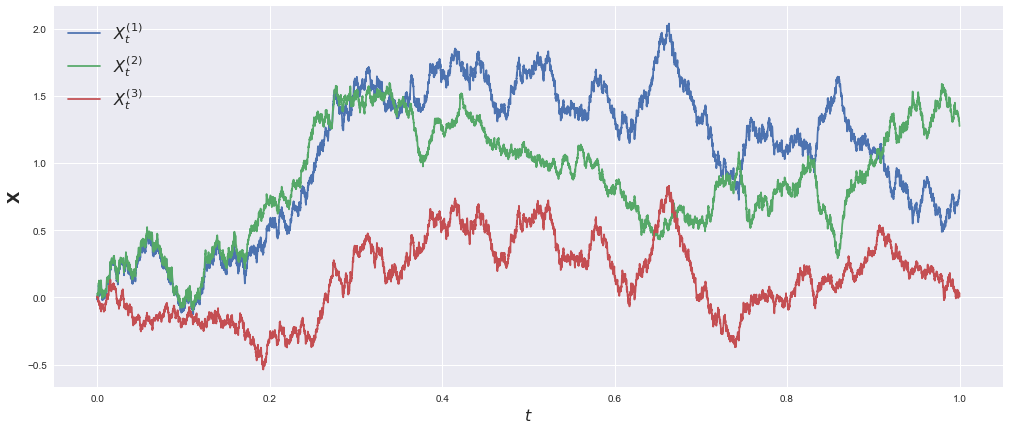
\includegraphics[scale=0.4]{X3}
			\caption{$\mathbf{X}_t$ from Example \ref{exmp X3}}
			\smallskip
			\small
			One can observe that $X_t^{(1)}$ and $X_t^{(2)}$ have strong positive correlation in the beginning, which decreases over time and later, when $t$ approaches $1$, turns into negative one. Meanwhile $X_t^{(3)}$ has independent fluctuations on the borders, but in the middle it repeats the behavior of $X_t^{(1)}$.
		\end{center}
	\end{figure}
	
	\begin{rmrk} \label{stoch calc notions}
		Recall the basic notions from the theory of stochastic calculus (w.l.o.g. we assume that all the processes have a starting point at $0$ a.s.):
		\begin{enumerate}
			\item An Itô process $X_t$ is defined to be an adapted stochastic process that can be expressed as the sum of an integral with respect to time and an integral with respect to Brownian motion:
			\[ X_t = \int_{0}^{t} \mu_s ds + \int_{0}^{t} \sigma_s dW_s. \]
			\item Let $X$ be a continuous local martingale. Then $[X]_t$ with
			\[ [X]_t = X_t^2 - 2 \int_0^t X_sdX_s \]
			is called \define{quadratic variation} of $X$.
			\item The \define{quadratic covariation} of two continuous semimartingales $X$ and $Y$ is defined as follows:
			\[ [X, Y]_t = \frac{1}{4}([X + Y]_t - [X-Y]_t). \]
			\item Let $X$ and $Y$ be Itô processes with volatilities ${\sigma_X}_t$ and ${\sigma_Y}_t$ with respect to the same Brownian motion, then
			\[ [X, Y]_t = \int_0^t {\sigma_X}_s{\sigma_Y}_s ds. \]
			\item Quadratic covariation is symmetric and bilinear map:
			\[ [X + Y, Z]_t = [X, Z]_t + [Y, Z]_t, \]
			\[ [X, Y + Z]_t = [X, Y]_t + [X, Z]_t, \]
			\[ [X, Y]_t = [Y, X]_t, \quad [X]_t = [X, X]_t \]
		\end{enumerate}
	\end{rmrk}
	
	\begin{exmp} \label{quad var}
		Let us consider two-dimensional case with $\mu_t = ({\mu_X}_t, {\mu_Y}_t)^T$ and
		\[\Theta_t = \begin{pmatrix}
		{\sigma_X}_t & \rho_t \\
		\rho_t & {\sigma_Y}_t
		\end{pmatrix} \]
		Then $\mathbf{X}_t = (X_t, Y_t)^T$, where 
		\[X_t = \int_0^t{\mu_X}_s ds + \int_0^t{\sigma_X}_s dW_s^{(1)} + \int_0^t\rho_s dW_s^{(2)}\] 
		and
		\[Y_t = \int_0^t{\mu_Y}_s ds + \int_0^t\rho_s dW_s^{(1)} + \int_0^t{\sigma_Y}_s dW_s^{(2)}.\]
		
		Using Remark \ref{stoch calc notions} we get
		\begin{equation}
			[X]_t = \int_{0}^{t}({\sigma_X}_s^2 + \rho_s^2) ds, \quad  [Y]_t = \int_{0}^{t}({\sigma_Y}_s^2 + \rho_s^2) ds
		\end{equation}
		and
		\begin{equation} \label{quadratic variation Ito}
         	[X, Y]_t = \int_{0}^{t}({\sigma_X}_s + {\sigma_Y}_s)\rho_s ds. 
		\end{equation}
		Let us look at the quadratic covariation $[X, Y]_1$ at time $1$. It is defined as follows: let $\Pi = \{ \tau_0, \dots, \tau_n \}$ be a partition of $[0, 1]$ (i.e. $0 = \tau_0 < \tau_1 < \dots \tau_n = 1$) and set up the sampled cross variation
		\begin{equation} \label{cross variation}
			\sum_{\ell = 1}^{n} \Delta X_\ell \Delta Y_\ell.
		\end{equation}
		Now let the number of partition points $n$ go to infinity as the length of the longest subinterval $\| \Pi \| = \max_{1 \leq \ell \leq n}(\tau_{\ell} - \tau_{\ell-1}) $ goes to zero. The sum in \eqref{cross variation} converges in probability to $[X, Y]_1$. This limit is given by the right-hand side of \eqref{quadratic variation Ito}. This assertion follows from the standard theorems in stochastic calculus. Writing formally,
		\[  \lim_{n \rightarrow \infty} \sum_{\ell = 1}^{n} \Delta X_\ell \Delta Y_\ell \xrightarrow{\mathbb{P}} [X, Y]_1. \]
		Hence,
		\[
		\lim_{n \rightarrow \infty} \sum_{\ell=1}^{n}\Delta \mathbf{X}_\ell(\Delta \mathbf{X}_\ell)^T
		= \lim_{n \rightarrow \infty} \sum_{\ell=1}^{n}\begin{pmatrix}
		(\Delta X_\ell)^2 & \Delta X_\ell \Delta Y_\ell \\
		\Delta Y_\ell \Delta X_\ell & (\Delta Y_\ell)^2
		\end{pmatrix} 
		\xrightarrow{\mathbb{P}} 
		\begin{pmatrix}
		[X]_1 & [X, Y]_1 \\
		[Y, X]_1 & [Y]_1
		\end{pmatrix}.
		 \]
		
		On the other hand,
		\[ \Theta_t^2 = \begin{pmatrix}
		{\sigma_X}_t^2 + \rho_t^2 & ({\sigma_X}_t + {\sigma_Y}_t)\rho_t \\
		({\sigma_X}_t + {\sigma_Y}_t)\rho_t  & {\sigma_Y}_t^2 + \rho_t^2
		\end{pmatrix}, \]
		and therefore we conclude that
		\[ \lim_{n \rightarrow \infty} \Sigma_2^{RCV} \xrightarrow{\mathbb{P}} \Sigma_2. \]
		
		The convergence of realized covariance to ICV  can be generalized for arbitrary $p$:
		\[  \lim_{n \rightarrow \infty} \sum_{\ell=1}^{n}\Delta \mathbf{X}_\ell(\Delta \mathbf{X}_\ell)^T \xrightarrow{\mathbb{P}} [\mathbf{X}, \mathbf{X}]_{p \times p}, \]
		where 
		\[[\mathbf{X}, \mathbf{X}]_{ij} = [X^{(i)}, X^{(j)}].\]
		(MORE DETAILS FOR GENERAL p HERE)
		Therefore,
		\[ \lim_{n \rightarrow \infty} \Sigma_p^{RCV} \xrightarrow{\mathbb{P}} \Sigma_p. \]
	\end{exmp}
	
	\pagebreak
	\part{Marchenko-Pastur law}
	\begin{rmrk}
		In Remark \ref{quad var} we claimed the convergence of RCV matrix to ICV for any finite $p$. In practice, however, it might be the case that the number of processes is approximately equal to the number of observations for each process. Theoretically, the problem arises when the value of $p$ has at least the same rate of growth as $n$. In this case the convergence is not well defined, because the RCV matrix has the unlimited size. Then, instead of consideration of the whole RCV matrix, we choose another criteria.
	\end{rmrk}
	
	\begin{defn}
		Let $\{\lambda_j:j=1,\dots, p\}$ be set of eigenvalues of ICV, then
		\[F^{\Sigma_p}(x) := \frac{\#\{j:\lambda_j \leq x\}}{p}, \quad x \in \MR, \]
		is called \define{empirical spectral distribution (ESD)}.
	\end{defn}
	
	\begin{prps} [Theorem 1.1 of Silverstein (1995)] \label{MP law} \
		\begin{enumerate}
			\item for $p = 1, 2, \dots$ and for $1 \leq \ell \leq n$, $\mathbf{Z}_\ell^{(p)} = (Z_\ell^{(p,j)})_{1 \leq j \leq p}$ with $Z_\ell^{(p,j)}$ i.i.d. with mean 0 and variance 1;
			\item $n = n(p)$ with $y_n := p/n \rightarrow y > 0$ as $p \rightarrow \infty$;
			\item $\Sigma_p$ is a (possibly random) nonnegative definite $p \times p$ matrix such that its ESD $F^{\Sigma_p}$ converges a.s. in distribution to a probability distribution $H$ on $[0,\infty)$ as $p \rightarrow \infty$;
			\item $\Sigma_p$ and $\mathbf{Z}_\ell^{(p)}$ are independent.
		\end{enumerate}
		Let $\Sigma_p^{1/2}$ be the (nonnegative) square root matrix of $\Sigma_p$ and 
		\[S_p:= \frac{1}{n} \sum_{\ell=1}^{n} \Sigma_p^{1/2} \mathbf{Z}_\ell^{(p)}(\mathbf{Z}_\ell^{(p)})^T \Sigma_p^{1/2}.\]
		Then a.s. the ESD of $S_p$ converges in distribution to a probability distribution $F$, which is determined by $H$ in that its Stieltjes transform
		\[ m_F(z):=\int_{\lambda \in \MR} \frac{1}{\lambda - z} dF(\lambda), \quad z \in \mathbb{C}_+ := \{ z \in \mathbb{C} : \Im(z)>0 \} \]
		solves the equation
		\begin{equation}
		m_F(z) = \int_{\tau \in \MR} \frac{1}{\tau (1-y(1+zm_F(z))) - z } dH(\tau).
		\end{equation}
	\end{prps}
	
	\begin{rmrk} \
		\begin{enumerate}
			\item Note that if $y \rightarrow 0$ limiting distribution function $F$ of $S_p$ matches limiting distribution function $H$ of $\Sigma_p$. This is the case, when $n$ grows faster than $p$ and as we stated before $\Sigma_p^{RCV}$ converges to $\Sigma_p$. 
			\item In the special case when $\Sigma_p = \sigma^2 \mathbb{I}_{p \times p}$, where $\mathbb{I}_{p \times p}$ is the $p \times p$ identity matrix, the LSD $F$ has an analytical expression, which can be derived from the following proposition.
		\end{enumerate}
	\end{rmrk}
	
	\begin{prps}[see, e.g., Theorem 2.5 in Bai (1999)]
		Suppose that $\mathbf{Z}_\ell^{(p)}$'s are as in the previous proposition, and $\Sigma_p = \sigma^2 \mathbb{I}_{p \times p}$ for some $\sigma^2>0$. Then the LSD $F$ has density
		\[ f(x) = \Big(1-\frac{1}{y}\Big)_+\delta_0(x) + \frac{1}{2 \pi \sigma^2 xy} \sqrt{(b-x)(x-a)} \mathbf{1}_{[a,b]}(x), \]
		where 
		\[ a = \sigma^2(1-\sqrt{y})^2 \quad \text{and} \quad b = \sigma^2(1+\sqrt{y})^2, \]
		and $\delta_0(x)$ is a Dirac delta function.
	\end{prps}
	The LSD $F$ in this proposition is called the Marchenko-Pastur law with ratio index $y$ and scale index $\sigma^2$, and will be denoted by $\mathcal{MP}(y, \sigma^2)$.
	\begin{figure}
		\begin{center} \centering
			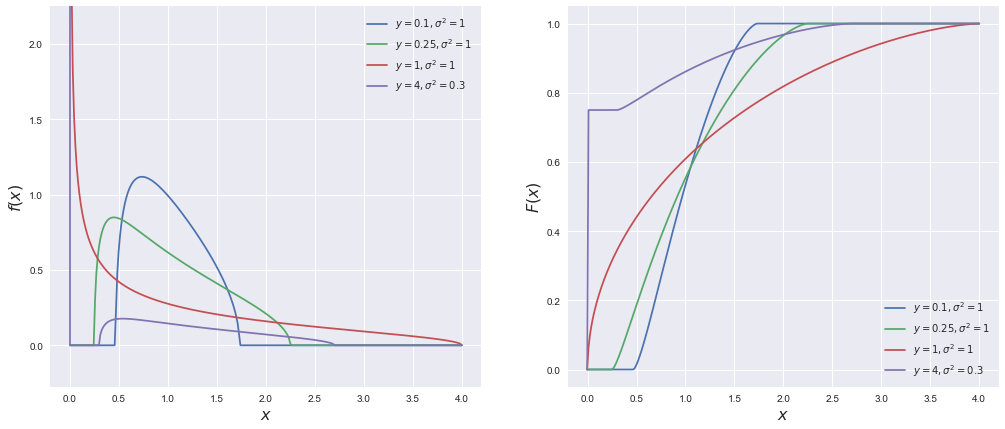
\includegraphics[scale=0.4]{MP}
			\caption{Marchenko-Pastur law}
		\end{center}
	\end{figure}
	
	\begin{rmrk}
		Let us set
		\[ \Theta_t^0 = \sqrt{\int_0^1\Theta_s^2 ds} \quad \forall t \in [0, 1] \]
		and corresponding matrix $\mathbf{X}_t^0$, such that
		\[ d\mathbf{X}_t^0 = \Theta_t^0d\mathbf{W}_t. \]
		Note that $\mathbf{X}_t$ and $\mathbf{X}_t^0$ share the same ICV matrix:
		\[ \Sigma_p^0 :=  \int_0^1(\Theta_t^0)^2 dt = \int_0^1 dt \int_0^1 \Theta_s^2 ds = \Sigma_p.  \]
		Based on $\mathbf{X}_t^0$, we have an associated RCV matrix
		\[ \Sigma_p^{RCV^0} = \sum_{\ell=1}^{n} \Delta \mathbf{X}_\ell^0 (\Delta \mathbf{X}_\ell^0)^T. \]
		Since $\Sigma_p^{RCV}$ and $\Sigma_p^{RCV^0}$ are based on the same estimation method and share the same targeting ICV matrix, it is desirable that their ESDs have similar properties. \\
		... bla bla bla discuss convergence and conclude that we can show that RCV may not converge in non-constant volatility case.
	\end{rmrk}
	
	\begin{lmm}[Weyl's Monotonicity Theorem]
		Suppose $A$ and $B$ are symmetric, $p \times p$ matrices. Let $\lambda_i(A)$ be the $i$-th largest eigenvalue of $A$. If $A \preceq B$, then $\lambda_i(A) \leq \lambda_i(B)$ for all $i$, or, equivalently
		\[ F^B(x) \leq F^A(x) \quad \forall x \geq 0. \]
    \end{lmm}
    \begin{proof}
    	Corollary 4.3.3 in Horn and Johnson (1990)
    \end{proof}
		
	\begin{prps}
		Suppose that for all $p$, $\mathbf{X}_t=\mathbf{X}_t^{(p)}$ is a $p$-dimensional process satisfying
		\begin{equation}
		d \mathbf{X}_t = \gamma_t d\mathbf{W}_t, \quad t \in [0, 1],
		\end{equation}
		where $\gamma_t > 0$ is a nonrandom (scalar) c$\grave{\text{a}}$dl$\grave{\text{a}}$g process. Let $\sigma^2 = \int_0^1 \gamma_t^2 dt$ and so that the ICV matrix $\Sigma_p = \sigma^2 \mathbb{I}_{p \times p}$. Assume further that the observation times $\tau_{n,\ell}$ are equally spaced, that is, $\tau_{n, \ell} = \ell / n$, and that the RCV matrix $\Sigma_p^{RCV}$ is defined by \eqref{RCV}. Then so long as $\gamma_t$ is not constant on $[0, 1)$, for any $\varepsilon > 0$, there exists $y_c = y_c(\gamma, \varepsilon) > 0$ such that if $\lim p/n = y \geq y_c$,
		\begin{equation}
			\limsup F^{\Sigma_p^{RCV}}(b(y)+\sigma^2\varepsilon) < 1 \quad a.s.
		\end{equation}
		In particular, $F^{\Sigma_p^{RCV}}$ doesn't converge to the Marchenko-Pastur law $\mathcal{MP}(y, \sigma^2)$.
    \end{prps}
    
    \begin{proof}
    	By assumption if $\gamma_t$ is non-contant, there exists $\delta > 0$ and an interval $[c, d] \subseteq [0, 1] $ such that
    	\[ \gamma_t \geq \sigma(1+\delta) \quad \forall t \in [c, d]. \]
    	Therefore, if $\big[ \frac{\ell - 1}{n}, \frac{\ell}{n} \big] \subseteq [c, d] $ for some $1 \leq \ell \leq n$, then
    	\[ \Delta \mathbf{X}_\ell (\Delta \mathbf{X}_\ell )^T \stackrel{d}{=} \int_{(\ell-1)/n}^{\ell/n} \gamma_t^2 dt \cdot \mathbf{Z}_\ell(\mathbf{Z}_\ell)^T \succeq \frac{(1+\delta)^2}{n} \sigma^2 \mathbf{Z}_\ell(\mathbf{Z}_\ell)^T,  \]
    	where $\mathbf{Z}_\ell = (Z_\ell^{(1)}, \dots , Z_\ell^{(p)})^T$ consists of independent standard normals. Hence, if we let $ J_n = \big\{ \ell: \big[ \frac{\ell - 1}{n}, \frac{\ell}{n} \big] \subseteq [c, d] \big\} $ and
    	\[ \Gamma_p = \sum_{\ell \in J_n} \Delta \mathbf{X}_\ell (\Delta \mathbf{X}_\ell )^T, \quad \Lambda_p = \frac{\sigma^2}{n(d-c)} \sum_{\ell \in J_n} \mathbf{Z}_\ell (\mathbf{Z}_\ell )^T,  \]
    	then for any $x \geq 0$, by Weyl's Monotonicity Theorem,
    	\[
    	F^{\Sigma_p^{RCV}}(x) \leq F^{\Gamma_p}(x) \leq F^{\Lambda_p}\bigg(\frac{x}{(1+\delta)^2(d-c)}\bigg).
    	\]
	    Now note that $\# J_n \sim (d-c)n$, hence if $p/n \rightarrow y$, by Proposition \ref{MP law}, $F^{\Lambda_p}$ will converge a.s. to the Marchenko-Pastur law with ratio index $y'=\frac{y}{d-c}$ and scale index $\sigma^2$.
	    By the formula of $b(\cdot)$ in Marchenko-Pastur density
	    \[
	    \begin{aligned}
	    (1+\delta)^2(d-c)b(y') &=(1+\delta)\sigma^2 \cdot (1+\delta)(d-c)(1+2\sqrt{y'}+y') \\
	    & =(1+\delta)\sigma^2 \cdot (1+\delta)(d-c + 2\sqrt{(d-c)y} + y) \\
	    & := (1+\delta)\sigma^2 \cdot  g(y).
	    \end{aligned}
	    \]
	    Note that the $g(y)$ has a linear growth in $y$ with coefficient $1+\delta$. Hence, for any $\varepsilon > 0$, there exists $y_c > 0$, such that for all $y \geq y_c$
	    \[ g(y) \geq (1+\sqrt{y})^2+\varepsilon,  \]
	    that is,
	    \[ (1+\delta)^2(d-c)b(y') \geq (1+\delta) \sigma^2 \cdot ((1+\sqrt{y})^2+\varepsilon) = (1+\delta)(b(y)+\sigma^2\varepsilon)  \]
	    or, equivalently,
	    \[ \frac{b(y) + \sigma^2\varepsilon}{(1+\delta)^2(d-c)} \leq \frac{b(y')}{1+\delta}. \]
	    Therefore, when the above inequality holds,
	    \[\limsup F^{\Sigma_p^{RCV}}(b(y) + \sigma^2\varepsilon) \leq \limsup F^{\Lambda_p}\bigg(\frac{b(y')}{1+\delta}\bigg) < 1. \]
    \end{proof}
    
    \pagebreak
    \part{Limiting theorems for non-constant covolatility process}
    
    \begin{rmrk}
    	Firstly let us explain to which law RCV can converge...
    \end{rmrk}
    
    \begin{thm} \label{Thm 1}
    	Assume that all the conditions in Proposition \ref{MP law} are satisfied. Furthermore,
    	\begin{enumerate}
    		\item $Z_\ell^{(p, j)}$ have finite moments of all orders;
    		\item $H$ has a finite second moment;
    		\item the weights $w_\ell^n$, $1 \leq \ell \leq n$, $n = 1, 2, \dots$, are all positive, and there exists $\kappa < \infty$ such that the rescaled weights $(nw_\ell^n)$ satisfy
    		\[ \max_n \max_{\ell = 1, \dots, n} (nw_\ell^n) \leq \kappa; \]
    		moreover, almost surely, there exists a c$\grave{\text{a}}$dl$\grave{\text{a}}$g function $w_s: [0, 1] \rightarrow \MR_{+}$, such that
    		\[ \lim_n \sum_{1 \leq \ell \leq n} \int_{(\ell-1)/n}^{\ell/n} |n w_\ell^n - w_s|ds = 0; \]
    		\item there exists a sequence $\eta_p = o(p)$ and a sequence of index sets $\mathcal{I}_p$ satisfying $\mathcal{I}_p \subset \{1, \dots, p\}$ and $\#\mathcal{I}_p \leq \eta_p$ such that for all $n$ and all $\ell$, $w_\ell^n$ may depend on $\mathbf{Z}_\ell^{(p)}$ but only on $\{ Z_\ell^{(p,j)}: j \in \mathcal{I}_p \}$;
    		\item there exist $C < \infty$ and $\delta < 1/6$ such that for all $p$, $\| \Sigma_p \| \leq Cp^\delta$ a.s.
    	\end{enumerate}
    	Define $S_p = \sum_{\ell=1}^{n} w_\ell^n \cdot \Sigma_p^{1/2} \mathbf{Z}_\ell^{(p)} (\mathbf{Z}_\ell^{(p)})^T\Sigma_p^{1/2} $. Then, almost surely, the ESD of $S_p$ converges in distribution to a probability distribution $F^w$, which is determined by $H$ and $(w_s)$ in that it Stiltjes trasform $m_{F^w}(z)$ is given by
    	\[ m_{F^w}(z) = -\frac{1}{z} \int_{\tau \in \MR} \frac{1}{\tau M(z) + 1} dH(\tau), \]
    	where $M(z)$, together with another function $\tilde{m}(z)$, uniquely solve the following equation in $\mathbb{C}_{+} \times \mathbb{C}_{+}$:
    	\[
    	\left \{
    	\begin{array}{l}
    		M(z) = -\frac{1}{z} \int_{\tau \in \MR} \frac{w_s}{1 + y \tilde{m}(z)w_s} ds,  \\
    		\tilde{m}(z) =  -\frac{1}{z} \int_{\tau \in \MR} \frac{\tau}{\tau M(z) + 1} dH(\tau).
    	\end{array}
    	\right.
    	\]
    \end{thm}
    
    \begin{rmrk}
    	If $w_\ell^n = 1/n$, then $w_s=1$, and Theorem \ref{Thm 1} reduces to Proposition \ref{MP law}. Moreover, if $w_s$ is not constant, that is, $w_s \neq \int_{0}^{1} w_t dt$ on $[0, 1]$, then except in the trivial case when $H$ is a delta measure at $0$, the LSD $F^w \neq F$, where $F$ is the LSD in Proposition \ref{MP law} determined by $H(\cdot / \int_{0}^{1} w_t dt)$. (ADD MORE EXPLANATION FROM SUPPLEMENTARY ARTICLE)
    \end{rmrk}
    
    \begin{defn}
   		Suppose that $\mathbf{X}_t$ is a $p$-dimensional process satisfying \eqref{X diffeq}, and $\Theta_t$ is c$\grave{\text{a}}$dl$\grave{\text{a}}$g. We say that $\mathbf{X}_t$ belongs to \define{class $\mathcal{C}$} if, almost surely, there exist $\gamma_t: [0, 1] \mapsto \MR$ and $\Lambda$ a $p \times p$ matrix satisfying $\tr(\Lambda \Lambda^T) = p$ such that 
   		\begin{equation} \label{class C cov}
   		\Theta_t = \gamma_t \Lambda.
   		\end{equation}
   		Observe that if \eqref{class C cov} holds, then the ICV matrix $\Sigma_p = \int_{0}^{1} \gamma_t^2 dt \cdot \Lambda \Lambda^T$. The special case when $\Lambda = \mathbb{I}_{p \times p}$ is studied in simulation studies. (STUDIED IN STUDIES???)
   	\end{defn}
    		
    \begin{exmp}
    	Suppose that $X_t^{(j)}$ satisfy
    		\[ dX_t^{(j)} = \mu_t^{(j)} dt + \sigma_t^{(j)}dW_t^{(j)}, \quad j = 1, \dots, p, \]
    		where $\mu_t^{(j)}, \sigma_t^{(j)} : [0, 1] \rightarrow \MR$ are the drift and volatility processes for stock $j$, and $W_t^{(j)}$'s are (one-dimensional) standard Brownian motions. If the following conditions hold:
    		\begin{itemize}
    			\item the correlation matrix process of $(W_t^{(j)})$
    			\[ R_t:= \bigg(\frac{ [W^{(j)}, W^{(k)}]_t \ }{t}\bigg)_{1 \leq j,k \leq p} =:(r^{(jk)})_{1 \leq j,k \leq p} \]
    			is constant in $t \in [0, 1]$.
    			\item $r^{(jk)} \neq 0$ for all $1 \leq j,k \leq p$; and
    			\item the correlation matrix process of $X_t^{(j)}$
    			\[ \Bigg( \frac{\int_{0}^{t} \sigma_s^{(j)}\sigma_s^{(k)} d[W^{(j)}, W^{(k)}]_s }{\sqrt{\int_{0}^{t} (\sigma_s^{(j)})^2 ds \cdot \int_{0}^{t} (\sigma_s^{(k)})^2 ds}} \Bigg)_{1 \leq j,k \leq p}  =:(\rho^{(jk)})_{1 \leq j,k \leq p}  \]
    			is constant in $t \in [0, 1]$;
    		\end{itemize}
    		then $\mathbf{X}_t$ belongs to class $\mathcal{C}$.
    		
    		\begin{proof}
    			For any $t \in [0, 1]$: 
    			\[ \rho^{(jk)} = \frac{r^{(jk)} \int_{0}^{t} \sigma_s^{(j)}\sigma_s^{(k)} ds }{\sqrt{\int_{0}^{t} (\sigma_s^{(j)})^2 ds \cdot \int_{0}^{t} (\sigma_s^{(k)})^2 ds}}, \]
    			therefore
    			\[ \frac{\rho^{(jk)}}{r^{(jk)}} = \frac{\int_{0}^{t} \sigma_s^{(j)}\sigma_s^{(k)} ds/t }{\sqrt{\int_{0}^{t} (\sigma_s^{(j)})^2 ds/t \cdot \int_{0}^{t} (\sigma_s^{(k)})^2 ds/t}}. \]
    			Letting $t \downarrow 0$, using l'H$\hat{\text{o}}$pital's rule and noting that $\sigma_t^{(j)}$ are c$\grave{\text{a}}$dl$\grave{\text{a}}$g, we observe that
    			\[ \frac{\rho^{(jk)}}{r^{(jk)}} = \frac{\sigma_0^{(j)}\sigma_0^{(k)}}{ \sqrt{  (\sigma_0^{(j)})^2 \cdot (\sigma_0^{(k)})^2 }} = \pm 1. \]
    			Hence, for all $t \in [0, 1]$:
    			\[ \bigg| \int_{0}^{t}\sigma_s^{(j)}\sigma_s^{(k)} ds \bigg| = \sqrt{\int_{0}^{t} (\sigma_s^{(j)})^2 ds \cdot \int_{0}^{t} (\sigma_s^{(k)})^2 ds} . \]
    			By Cauchy-Schwartz inequality, this holds only if $\sigma_s^{(j)}$ and $\sigma_s^{(k)}$ are proportional to each other. Therefore, almost surely, there exists a scalar process $\gamma_t : [0, 1] \rightarrow \MR$ and a $p$-dimensional vector $(\sigma^{(1)}, \dots, \sigma^{(p)})^T$, such that
    			\[ (\sigma_t^{(1)}, \dots, \sigma_t^{(p)})^T = \gamma_t \cdot (\sigma^{(1)}, \dots, \sigma^{(p)})^T. \]
    			Now we show that $\mathbf{X}_t$ belongs to class $\mathcal{C}$. In fact one can always find a $p$-dimensional standard Brownian motion $\widetilde{\mathbf{W}}_t$, such that 
    			\[ \mathbf{W}_t = R^{1/2}\widetilde{\mathbf{W}}_t, \]
    			where $\mathbf{W} = (W_t^{(1)}, \dots, W_t^{(p)})^T$ and $R$ is a correlation matrix of $\mathbf{W}_t$, which is constant for all $t \in [0, 1]$ by assumption. Hence, writing $\mu_t = (\mu_t^{(1)}, \dots, \mu_t^{(p)})^T$, we have
    			\[ d\mathbf{X}_t = \mu_t dt + \diag(\sigma_t^{(1)}, \dots, \sigma_t^{(p)}) d\mathbf{W}_t = \mu_t dt +\gamma_t \cdot \diag(\sigma^{(1)}, \dots, \sigma^{(p)}) R^{1/2} d\widetilde{\mathbf{W}}_t. \]
    		\end{proof}
    \end{exmp}
    
    \begin{rmrk}
    	The process in Example \ref{exmp X3} doesn't belong to the class $\mathcal{C}$, because its correlation structure varies in time.
    \end{rmrk}
    		
    \begin{defn}
   		Suppose that a diffusion process $\mathbf{X}_t$ belongs to class $\mathcal{C}$. We define \define{time-variation adjusted realized covariance (TVARCV) matrix} as follows:
   		\begin{equation} \label{TVARCV}
   		\widehat{\Sigma}_p := \frac{\tr \big( \Sigma_p^{RCV} \big) }{n} \sum_{\ell = 1}^{n} \frac{\Delta \mathbf{X}_\ell (\Delta \mathbf{X}_\ell)^T}{\| \Delta \mathbf{X}_\ell \|_2^2} = \frac{\tr \big( \Sigma_p^{RCV} \big) }{p} \widetilde{\Sigma}_p,
   		\end{equation}
   		where
   		\begin{equation} \label{Sigma_tilde}
   		\widetilde{\Sigma}_p := \frac{p}{n} \sum_{\ell = 1}^{n} \frac{\Delta \mathbf{X}_\ell (\Delta \mathbf{X}_\ell)^T}{\| \Delta \mathbf{X}_\ell \|_2^2}.
   		\end{equation}
    \end{defn}
    
    \begin{rmrk}
    	Let us explain $\widetilde{\Sigma}_p$. Consider the simplest case when $\mu_t = 0$, $\gamma_t$ deterministic, $\Lambda_t = \mathbb{I}_{p \times p}$, and $\tau_{n,\ell} = \ell / n$, $\ell = 0, 1, \dots, n$. In this case,
    	\[ \Delta \mathbf{X}_\ell = \sqrt{\int_{(\ell - 1)/n}^{\ell / n} \gamma_t^2 dt }\cdot \frac{\mathbf{Z}_\ell}{\sqrt{n}}, \]
    	where $\mathbf{Z}_\ell = (Z_\ell^{(1)}, \dots, Z_\ell^{(p)})^T$ is a vector of i.i.d. standard normal random variables. Hence,
    	\[ \frac{\Delta \mathbf{X}_\ell (\Delta \mathbf{X}_\ell)^T}{\| \Delta \mathbf{X}_\ell \|_2^2} = \frac{\mathbf{Z}_\ell \mathbf{Z}_\ell^T}{\|  \mathbf{Z}_\ell \|_2^2}. \]
    	However, as $p \rightarrow \infty$, $\| \mathbf{Z}_\ell \|_2^2 \sim p$, hence
    	\[ \widetilde{\Sigma}_p \sim \frac{\sum_{\ell = 1}^{n}\mathbf{Z}_\ell \mathbf{Z}_\ell^T}{n}, \]
    	the latter being the usual sample covariance matrix.
    	We will show that, first, $\tr(\Sigma_p^{RCV}) \sim \tr(\Sigma_p)$; and second, if $\mathbf{X}_t$ belongs to class $\mathcal{C}$ and satisfies certain additional assumptions, then the LSD of $\widetilde{\Sigma}_p$ is related to that of $OHLALAL$ via the Marchenko-Pastur equation, where
    	\[ OHLALAA \]
    	Hence, the LSD of $\widehat{\Sigma}_p$
    \end{rmrk}
    
    \begin{thm} \label{Thm 2}
    	Let's state the assumptions:
    	\begin{enumerate}
    		\item there exists $C_0 < \infty$ such that for all $p$ and all $j = 1, \dots, p$, $|\mu_t^{(p,j)}| \leq C_0$ for all $t \in [0, 1]$ a.s.;
    		\item there exist constants $C_1 < \infty$, $0 \leq \delta_1 < 1/2$, a sequence $\eta_p < C_1 p^{\delta_1}$ and a sequence of index sets $\mathcal{I}_p$ satisfying $\mathcal{I}_p \subset \{ 1, \dots p \}$ and $\# \mathcal{I}_p \leq \eta_p$ such that $\gamma_t^{(p)}$ may depend on $\mathbf{W}_t^{(p)}$ but only on $\{ W_t^{(p, j)} : j \in \mathcal{I}_p \}$; moreover, there exists $C_2 < \infty$ such that for all $p$, $|\gamma_t^{(p)}| \in (1/C_2, C_2)$ for all $t \in [0, 1]$ a.s.;
    		\item there exists $C_3 < \infty$ such that for all $p$ and for all $j$, the individual volatilities \[ \sigma_t^{(j)} = \gamma_t^{(p)}\sqrt{\sum_{k=1}^{p} (\Lambda_{jk}^{(p)})^2} \in (1/C_3, C_3)\] for all $t \in [0, 1]$ a.s.;
    		\item \[ \lim_{p \rightarrow \infty} \frac{\tr(\Sigma_p)}{p} = \lim_{p \rightarrow \infty} \int_{0}^{1} (\gamma_t^{(p)})^2 dt := \theta > 0 \quad a.s.; \]
    		\item almost surely, as $p \rightarrow \infty$, the ESD $F^{\Sigma_p}$ converges to a probability distribution $H$ on $[0, \infty)$;
    		\item there exist $C_5 < \infty$ and $0 \leq \delta_2 < 1/2$ such that for all $p$, $\| \Sigma_p \| \leq C_5 p^{\delta_2}$ a.s.;
    		\item the $\delta_1$ in (ii) and $\delta_2$ in (vi) satisfy that $\delta_1 + \delta_2 < 1/2$;
    		\item $p/n \rightarrow y \in (0, \infty) $ as $p \rightarrow \infty$; and
    		\item there exists $C_4 < \infty$ such that for all $n$,
    		\[ \max_{1 \leq \ell \leq n} n \cdot (\tau_{n, \ell} - \tau_{n, \ell - 1}) \leq C_4 \quad a.s.  \]
    		moreover, $\tau_{n, \ell}$'s are independent of $\mathbf{X}_t$.
    	\end{enumerate}    
    		Suppose that for all $p$, $\mathbf{X}_t = \mathbf{X}_t^{(p)}$ is a $p$-dimensional process in class $\mathcal{C}$ for some drift process $\mu_t^{(p)} = (\mu_t^{(p, 1)}, \dots , \mu_t^{(p, p)})^T$, covolatility process $\Theta_t^{(p)} = \gamma_t^{(p)} \Lambda^{(p)}$ and a $p$-dimensional Brownian motion $\mathbf{W}_t^{(p)}$, which satisfy (i)-(vii) above. Suppose also that $p$ and $n$ satisfy (viii), and the observation times satisfy (ix). Let $\hat{\Sigma}_p$ be as in \eqref{TVARCV}. Then, as $p \rightarrow \infty$, $F^{\hat{\Sigma}_p}$ converges a.s. to a probability distribution $F$, which is determined by $H$ through Stieltjes transforms via the same Marchenko-Pastur equation as in Proposition \ref{MP law}.
    \end{thm}
    \begin{proof}
    	содержимое...
    \end{proof}
    
    
    \pagebreak
    \part{Simulation studies}
    
    \begin{exmp} \label{SimCos}
    	Let's take an example from the paper...
    	\[ \gamma_t = \sqrt{0.0009 + 0.0008 \cos(2 \pi t)}. \]
    	Then
    	\[ \sigma^2 = \int_{0}^{1}(0.0009 + 0.0008 \cos(2 \pi t)) dt = 0.0009. \]
    \end{exmp}
    
    \begin{figure}
    	\begin{center} \centering
    		\includegraphics[scale=0.4]{XCos}
    		\caption{ $\mathbf{X_t}$ from Example \ref{SimCos}, $n = 1000$, $p=1000$ }
    		\smallskip
    		\small
    		In this setting $y = p/n = 1$...
    	\end{center}
    \end{figure}
    
    \begin{figure}
    	\begin{center} \centering
    		\includegraphics[scale=0.4]{XCos2}
    		\caption{ $\mathbf{X_t}$ from Example \ref{SimCos}, $n = 1000$, $p=4000$ }
    		\smallskip
    		\small
    		In this setting $y = p/n = 4$...
    		Note point mass equal to $0.75$ at the origin.
    	\end{center}
    \end{figure}
    
    \begin{defn} \
    	\begin{enumerate}
    		\item 
    		The stochastic process $Y_t$ is called \define{Cox-Ingersoll-Ross (CIR) process}, if it is determined by the stochastic differential equation (SDE):
    		\begin{equation} \label{CIR}
    		    dY_t = \beta(\alpha - Y_t)dt + \xi\sqrt{Y_t}d \overline{W}_t,
    		\end{equation}
    		where $\alpha$, $\beta$ and $\xi$ are positive constants, and $\overline{W}_t$ is a standard Brownian motion. Conditional on parameters and initial value $Y_0$, scaled CIR process has a non-central chi-squared distribution with $k$ degrees of freedom and non-centrality parameter $\lambda$:
    		\[ c Y_t \sim {\chi'}_k^2(\lambda),  \]
    		where
    		\[k = \frac{4\alpha \beta}{\xi^2},\ \lambda = Y_0 c \exp^{-\beta t} \text{ and } c = \frac{4 \beta}{\xi^2 (1-\exp^{-\beta t})}.\]
    		\item The basic \define{Heston model} assumes that one-dimensional log-price process $X_t$ is determined by the following SDE:
    		\begin{equation} 
    		dX_t = \mu dt + \sqrt{Y_t}d\widetilde{W}_t,
    		\end{equation}
    		where $Y_t$ satisfies SDE \eqref{CIR} and $\widetilde{W}_t$ is another standard Brownian motion, such that 
    		\begin{equation} \label{dependent Brownian}
    		[\widetilde{W}, \overline{W}]_t = \int_{0}^{t}\rho_s ds
    		\end{equation}
    		holds with a (stochastic) process $\rho_t$, taking values strictly between $-1$ and $1$. Sometimes equality \eqref{dependent Brownian} is informally written as
    		\[ d\widetilde{W}_td\overline{W}_t = \rho_t dt. \]
    	\end{enumerate}
    \end{defn}
    
    \begin{exmp} \label{SimCIR}
    	Let's assume
    	\[ \gamma_t = \sqrt{Y_t}, \]
    	where $Y_t$ is a CIR process, determined by \eqref{CIR}. Then it is easy to show that
    	\[ \sigma^2 = \beta\alpha - \beta\int_{0}^{1} \gamma_t^2dt + \xi \int_{0}^{1} \gamma_t dW_t.\]
    	Moreover, let
    	\[ \overline{W}_t = \frac{1}{\sqrt{\eta_p}} \sum_{j=1}^{\eta_p}W_t^{(j)}, \]
    	where $\eta_p$ is determined by assumption (ii) in Theorem \ref{Thm 2}.
    	For any $0 \leq i \leq p$ we have:
    	\[ dW_t^{(i)}\cdot d\overline{W}_t = dW_t^{(i)} \cdot \frac{1}{\sqrt{\eta_p}} \sum_{j=1}^{\eta_p}dW_t^{(j)} = \frac{dt}{\sqrt{\eta_p}} \mathbf{1}_{\{i \leq \eta_p\}}, \]
    	or equivalently 
    	\[ [W^{(i)}, \overline{W}]_t =  \frac{t}{\sqrt{\eta_p}} \mathbf{1}_{\{i \leq \eta_p\}}.  \]
    \end{exmp}
    
    \begin{figure}
    	\begin{center} \centering
    		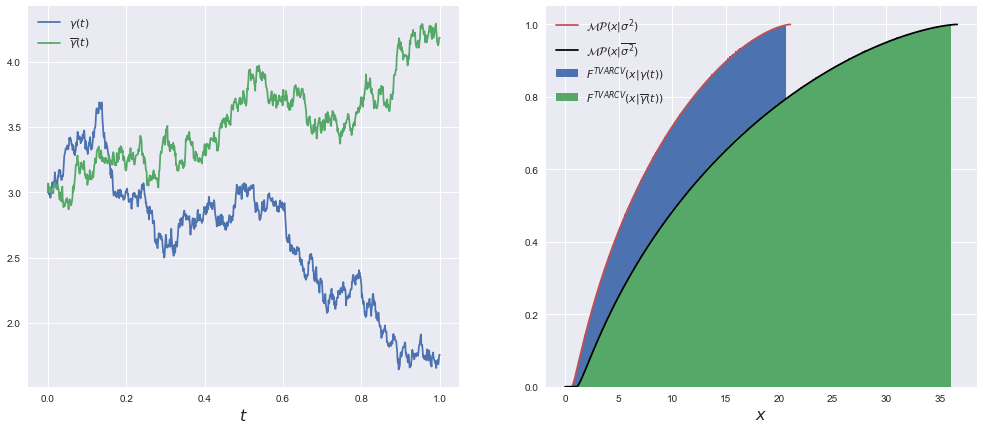
\includegraphics[scale=0.4]{XCIR}
    		\caption{$\eta_p = p, y = 0.5, \alpha = 1, \beta = 2, \gamma_0 = 10, \xi = 10$}
    	\end{center}
    \end{figure}
    
    
    \pagebreak
    \part{Conclusion}
    
\end{document}
